\documentclass[journal, a4paper]{IEEEtran}

\usepackage{graphicx}   % Written by David Carlisle and Sebastian Rahtz


\usepackage{url}        % Written by Donald Arseneau

\usepackage{amsmath}    % From the American Mathematical Society
\usepackage{amssymb}

\usepackage[utf8]{inputenc}

\usepackage{subcaption}

\usepackage{listings}
% \usepackage[title]{appendix}

\usepackage{color}


\definecolor{mygray}{rgb}{0.8,0.8,0.8}
\definecolor{mygreen}{rgb}{0,0.7,0.5}
\definecolor{myorange}{rgb}{1.0,0.4,0}

\definecolor{codegreen}{rgb}{0,0.6,0}
\definecolor{codegray}{rgb}{0.5,0.5,0.5}
\definecolor{codepurple}{rgb}{0.58,0,0.82}
\definecolor{backcolour}{rgb}{0.95,0.95,0.92}

\lstset{
basicstyle=\ttfamily\footnotesize,
commentstyle=\color{mygray},
numbers=left,
numbersep=2pt,
numberstyle=\tiny\color{mygray},
keywordstyle=\color{codepurple},
showspaces=false,
showstringspaces=false,
stringstyle=\color{myorange},
tabsize=2,
breakatwhitespace=true,
breaklines=true,
}


\begin{document}

\title{IDMT Final project 2018: Boidsong}
\author{Chris Yeoward}
\maketitle

\section*{Introduction}
Inspired by the murmuration of starlings, I was interested in creating an interactive sonification of a flock of birds, being enjoyable to watch, listen to and play with throughout its endless evolution. I wanted to experiment with call and response musical improvisation, presenting the user with an easy interface with which to create melodies, and to have an interpretation of those melodies echoed back by the birds.

The idea to achieve this installation was then to have a sine oscillator associated with each bird, with the distance and position of the bird from the virtual viewpoint governing the amplitude and position of the sound source. The oscillators would have pitches relating to a particular musical scale, arbitrarily chosen as C Minor melodic spanning a number of octaves, to ensure musicality and avoid discordance. In itself, this would create an evolving ambient sound field, though one without structure or coherence. The user would then play a melody using a softsynth in the same key as the birds. The birds whose pitch matches that played by the user would then be drawn to the camera, increasing the volume of the oscillator above the level of the ambient noise and thus repeating the notes played. To add variation to the sounds, and uniqueness to each bird, a triangle wave LFO was assigned to the amplitude of each oscillator with a random frequency and duty cycle.


\section*{Technical evaluation}
The project started in Processing from a bundled example that implements Craig Reynolds flocking algorithm \cite{reynolds} in 2D, which I then adapted to three dimensions. With regards to scale, more birds is generally more interesting when it comes to flocking. However, this must be balanced against the number of oscillators, as too many could result in an overbearing amount of noise, and the technical limitations of the implementation. As such a number of 100 birds was chosen as a starting point. From this, the first challenge was to determine how best to render the 100 birds and oscillators concurrently. Knowing that Processing had a built-in sound library and synthesis engine, I initially created an oscillator alongside each bird, and used the bird's position to modulate the amplitude and panning. This implementation reached its limit very quickly, with 5 birds/oscillators being enough to start hearing jittering in the audio and a distorted signal. This was not suprising as Java is not known for its ability to optimise audio.
An implementation in p5.js was then attempted, as I suspected that WebAudio may peform better than the Java applet. Additionally, a hosted version of the installation would have been desirable, from a showcasing perspective. P5 did manage to support more oscillators than Processing, however when running a sketch in full screen it struggled to render the birds particularly quickly, and a visible decrease in performance was observed for any more than 40 birds. The third and ultimate implementation featured a combination of using Processing for the flocking graphics, with position dispatched over OSC to a Max patch that rendered the sine oscillators. Max could handle 200 oscillators (100 for the carrier oscillators and 100 for their amplitude modulation) without any issue, and Processing was also able to render 100 birds in full screen while dispatching their position data without any reduction in performance.

A diagram of the technical implementation is shown in figure \ref{fig:tech}.

\begin{figure}[hbt!]
    \centering
    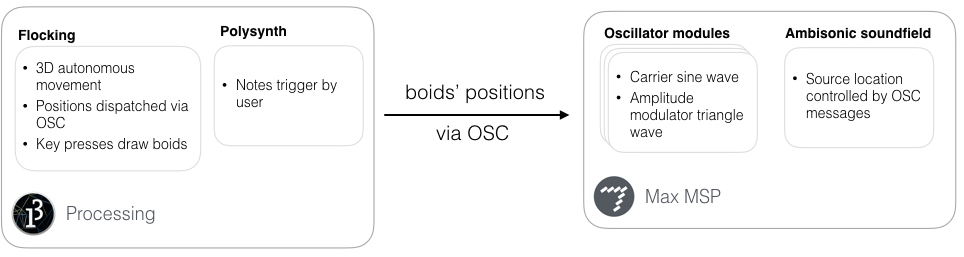
\includegraphics[width=\columnwidth]{tech_diag.jpeg}
    \caption{Technical solution.}
    \label{fig:tech}
\end{figure}

\section*{3D Rendering}
For rendering graphics in 2D Processing offers a useful method on its PVector class that calculates the heading of a vector, and returns the angle between the vector and the positive x axis. Then to orient a shape in two dimensions, only this one angle is required. In three dimensions however, 3 angles are needed to fully describe the orientation of a shape, known as Euler angles \cite{euler}. An alternative mathematical representation which is frequently used in videogames is the quaternion \cite{quaternion}, which rotates an object around a given vector. Neither of these approaches offered simple implementations in Processing, and as such it ultimately sufficed to draw the bird shape (shown in figure \ref{fig:boid}) in the direction of the normalised velocity vector. The orientation of the bird about the vector's axis was determined by the velocity differential such that the wings always were always perpendicular to the change in velocity. The velocity differential was used instead of the calculated acceleration as the velocity was always limited to be within a certain range. A vector parallel to the y axis was added to this velocity differential to flatten out the birds such that their turning and banking would appear more realistic, and to encourage their orientation to tend towards being along the x-y plane.

\begin{figure}[hbt!]
    \centering
    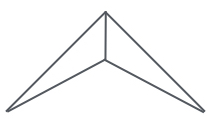
\includegraphics[width=0.4\columnwidth]{boid.jpeg}
    \caption{Boid shape.}
    \label{fig:boid}
\end{figure}

\section*{Flocking}
In its essence, the flocking algorithm provides an autonomous agent, known as a boid, with 3 simple rules for interacting with the rest of the flock \cite{reynolds}:
\begin{itemize}
  \item Cohesion: each boid determines the average position of each of its neighbours, and heads to that point
  \item Alignment: each boid determines the average velocity of each of its neighbours, and heads in that direction
  \item Separation: to avoid collisions, each boid will keep at a minimum distance from those around it
\end{itemize}

These few rules are applied as forces to each boid, and provide the basis for realistic flocking interactions of many forms, for birds, fish and mammals. Adjustment of their other characteristics can then fine tune the behaviour such that it represents the desired animal. In this instance, keeping the boids' velocity within a relatively small range, with a non-zero minimum limit, can produce more bird-like behaviours as they mimic the necessity for a bird to maintain momentum in the air. A fish, on the other hand, is able to change direction much faster than a bird, and can have a velocity of 0.
Traditionally, a boid is provided with a neighbourhood radius, within which it considers other boids as neighbours and updates its velocity accordingly, and a separation radius at which it will keep from other boids. This can create sharp changes in the acceleration vector as other boids move in and out of the radius threshold, which in this instance caused erratic rendering of the boids' wings. To avoid sudden changes, I set the force applied by the 3 rules to decrease with distance, as opposed to sharply dropping off outside of the radii. This also had the effect of attracting the boids to the average of all of their positions: the centre of the screen. To limit this behaviour, and to encourage fracturing within the group, I set the flocking rules only to be applied when a boid could 'see' the other boids, defined as being when another boid was in front of the boid in question.

\section*{Oscillator control}
Generating the audio required the creation of up to 100 oscillators in Max, controlled via the OSC protocol. In order to render these dynamically, I made use of the Max javascript patch, such that any number of oscillator patches could be created through sending a message to the script. This permitted the oscillator frequencies to be generated programmatically, with those for the carrier waves taken from an array of notes, and those for the amplitude modulation generated at random. Initially, each oscillator module contained a carrier wave, a triangular modulator wave, a gain control and a panning patch, which were all encapsulated in a subpatch with inlets to control the gain and panning and outlets for the stereo output. OSC messages containing the position of each bird were then received in Max, and used to set the amplitude and pan for each module.
To improve visual feedback to the user, I had wished to transmit OSC messages back to Processing such that each bird would pulse synchronously with the LFO amplitude modulation of the oscillator with which it was associated. I tried both streaming the amplitude modulation directly, and doing the oscillation in Processing and synchronising during runtime, though neither were suitable and left the visuals more distracting than helpful. Had both the audio and graphics been rendered in the same program they would have been simpler to synchronise.


\section*{Softsynth}
For the auditory feedback to the user, a polyphonic softsynth was created in Processing using the sound library. The range of the synth was equivalent to the range of pitches represented by the birds, which spanned 4 octaves from midi notes C2 to Bb5. Any lower and the sine waves were not discernible, higher and they were too piercing. The keys $a-j$ were assigned as the synthesiser keyboard as this offered the simple interface, and the octave changes were handled by the $<$ and $>$ keys.
A drawback to building the project across two applications was that any change in configuration of the notes, for example octave range or key, in Max or Processing required a manual change in the other application. Ideally, one would be the master, and the other the slave, such that any changes would be reflected across both applications.

\section*{Bird Interaction}
Control of the birds was relatively simple, as it merely required the addition of another force to the bird's acceleration. Upon key press, the synthesiser would sound, and a force would be applied to the bird whose pitch matched that of the synthesiser's, drawing it towards the user's viewpoint. This would in turn increase the volume of the sine wave associated to that particular bird, and the user would hear their note repeated again above the ambient noise. The force would cease to be applied to the bird once it had reached the viewpoint, then permitting it to return back to the flock.
Spacebar was assigned as a mechanism with which to retain birds, such that they would not return to the flock whilst it was held down. In this way, the user could create chords of the birds. At this point, having 100 birds and oscillators was helpful, as it meant that for each note of the 4 octave scale, there were 2 or 3 birds that also represented that pitch. One bird would be attracted for each press of a key, so if a user then pressed the same note more than once in the melody, each of the different birds would be attracted towards the user in turn.
To provide some visual feedback to the user, each bird was rendered with a different colour for each note of the scale, and brightness and saturation of the colour was increased whilst that bird was being drawn to the camera.

\section*{Ambisonic soundfield}
With all of the components to the installation assembled, the soundfield still lacked clarity, and it was hard to discern a bird's pitch while it was closer above the ambient noise of the rest of the flock. This led to an exploration of how to render a sound source in 3d space. The HoaLibrary \cite{hoa} for Max had suitable documentation and a number of examples both explaining ambisonics and how to use the patches. By sending the patch the radius from the listener of each source, and the angles of incidence, the sound field could be rendered binaurally for a specified order of ambisonics, in this instance 3. This dramatically improved the aesthetics of the ambient sound, and also the clarity of the birds moving towards the camera. The messages between the two applications were transmitted at a fast enough rate such that there was minimal lag between seeing a bird move and hearing it's sound move also.
The ambisonic sound field was only rendered for two dimensions, as with three the audio began to jitter. A third dimension may offer a greater level of immersion, but most likely only would only be a marginal improvement in comparison with the move from stereo sound to two dimensional ambisonics. A greater level of immersion would also be acheived by permitting the user to rotate the camera's position, possible with the use of VR and head tracking.

\section*{Technical skills acquired}
This project began with a deep dive into vectors and a refresher of vectors mathematics whilst learning about Craig Reynold's flocking algorithms. I learnt about Euler angles, quaternions and how to render objects in 3d space, in particular in Processing. I pushed p5.js to its limit, before becoming acquainted with Processing's sound library and then with Max MSP, utilising the js object in Max to dynamically create patches. I also picked up some knowledge of best practices with transmitting data via OSC to Max, and the differences between TCP/IP and UDP. Finally, I learnt about ambisonics, and their implementation in the HoaLibrary.


\begin{thebibliography}{1}

\bibitem{reynolds}
Craig Reynolds (1987)
\textit{Flocks, Herds, and Schools: A Distributed Behavioral Model}
Computer Graphics, 21

\bibitem{euler}
Weisstein, Eric W.
\textit{Euler Angles}
http://mathworld.wolfram.com/EulerAngles.html


\bibitem{quaternion}
Vince, John.
\textit{Quaternions for Computer Graphics}
http://mathworld.wolfram.com/EulerAngles.html
Springer-Verlag London

\bibitem{hoa}
Pierre Guillot, Eliott Paris, Julien Colafrancesco
\textit{HoaLibrary}
http://hoalibrary.mshparisnord.fr/en

\end{thebibliography}


%  \begin{appendices}
% \section*{Wiring Configuration}
% The final input and output setup for the Bela and the breadboard is shown in figure \ref{fig:wiring}
% \begin{figure}[hbt]
%     \centering
%       \includegraphics[width=\columnwidth]{drum-machine.jpg}
%     \caption{Wiring configuration for the drum machine.}
%     \label{fig:wiring}
% \end{figure}
%  \end{appendices}

\end{document}
